\documentclass[12pt]{article}

\usepackage{color}
\usepackage[utf8]{inputenc}
\usepackage{fullpage}
\usepackage{indentfirst}
\usepackage{graphicx}
\usepackage{graphicx}
\usepackage{amssymb, amsmath}
\usepackage[frenchb]{babel}



\usepackage[pdftex=true,
hyperindex=true,
colorlinks=true]{hyperref}



\newsavebox{\boiteremarque}
\newenvironment{remarque}{%
% clause begin
\begin{lrbox}{\boiteremarque}% début mise en boîte
\begin{minipage}{.8\textwidth}}{%
% clause end
\end{minipage}
\end{lrbox}% fin mise en boîte
% production de la boîte encadrée
\begin{center}
\fbox{\usebox{\boiteremarque}}
\end{center}}




\title{Génératrice portable \\ Construction d'une alimentation \\ stabilisée en tension portable}
\author{Jérôme GRARD}
\addtolength{\textwidth}{1cm}
\addtolength{\oddsidemargin}{-0,5cm}


\begin{document}


\maketitle
\thispagestyle{empty}

\begin{remarque}
	Ce document a pour but de présenter les travaux de recherche permettant de construire une
	alimentation stabilisée en tension portable. Cette alimentation a pour contraintes d'utiliser
	des pièces récupérées en priorité ---pour alléger les coûts--- et de fonctionner avec des
	piles AA (LR6) de sorte à pouvoir les remplacer facilement et à moindre coût.\newline
	\begin{center}
		Ce document a été édité en \LaTeX --- Diffusons le logiciel libre ! \newline
		Mes autres projets sur http://the-destiny.no-ip.org
	\end{center}
\end{remarque}

\newpage



\pagestyle{plain}
\setcounter{page}{1}
\tableofcontents


\newpage



\section{Schéma électronique}

\begin{figure}[!h]
        \centering
        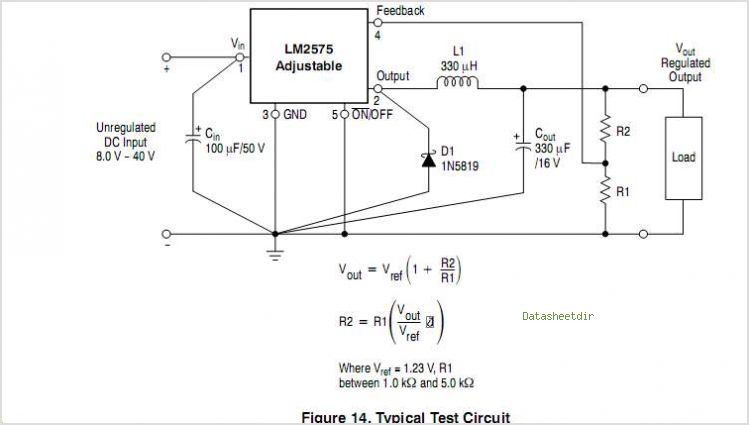
\includegraphics[scale=0.5]{Schema}
        \caption{Schema électronique}\label{Schema}
\end{figure}


\subsection{Choix}

Nous avons choisi la série LM 2575 pour deux raisons.

\begin{itemize}
	\item Alimentation à découpage
	\item Capable de délivrer une intensité de plus d'une ampère
\end{itemize}

Nous avons alors eu le choix entre plusieur modèles, le T ou le HV, de même que les composants stabilisés ou ajustable.
Le HV sert aux dispositifs ayant une grande plage de tensions en entrée, alors que le T est plus restreint. Compte tenu
de notre utilisation, nous prendrons donc un T\footnote{Le LM ne sera alimenté qu'avec des piles, dont la tension maximale
sera aux alentours de 12 / 13V.}. Concernant le choix entre un composant stabilisé ou ajustable, nous prendrons un ajustable
car cela figure dans la spécification initiale.


\subsection{Boitier}

Pour le boitier nous prendrons un TO 220, car il est plus facile à manipuler et permet la fixation d'un refroidisseur
passif. C'est de plus le plus facile à trouver dans le commerce.




\newpage
\section{Calculs}

Section détaillant tous les calculs des résistances nécessaire au paramétrage du module. Toutes les valeurs ici présentées
font référence au schéma \ref{Schema}.

\subsection{Valeur de R1}

Soit $R_2$ une résistance variable qui servira de commande à l'utilisateur pour modifier la tension de sortie, nous
avons $R_2$ tel que $R_2 \in [0.04 ; 31.6]  k\Omega$. Il faut donc utiliser la formule liant $R_2$, $R_1$, $V_{ref}$ et $V_{out}$.

\begin{equation}
	\boxed{V_{out} = V_{ref} \cdot (1 + \frac{R_2}{R_1})}
\end{equation}

Ici nous avons besoin d'atteindre 11V quand $R_2$ est au maximum. On va essayer de trouver le $R_1$ le plus
adapté en tenant compte des composants disponibles.
Nous utiliserons donc la fomrule dans cette forme\footnote{En rappellant que $V_{ref} = 1.23$ V} :

\begin{equation}
	\begin{split}
		R_1 = \frac{R_2 \cdot V_{ref}}{V_{out} - V_{ref}} & = \frac{31.6 \cdot 10^3 \times 1.23}{11 - 1.23} \\
								  & = 4.0 \cdot 10^3
	\end{split}
\end{equation}

Or nous avons à disposition des CMS Phycomp 8.2 $k\Omega$ à 1\%. Mis en parrallèle, nous avons donc 4.1 $k\Omega$. Cela
donne donc les résultats suivant :

\begin{align}
	V_{out Max}& = 10.71 V \\
	V_{out Min}& = 1.24 V
\end{align}


\subsection{Calibration à 5V}

On veut aussi avoir un mode calibré directement à 5V, sans avoir à faire de réglage. Un interrupteur permettra de
commuter les deux modes. Dans l'un  $R_2$ sera branchée, dans l'autre ce sera $R_{2bis}$ qui la remplacera. Nous
allons donc calculer $R_{2bis}$.

\begin{equation}
	\begin{split}
		R_{2bis} = R_1 \cdot ( \frac{V_{stab}}{V_{ref}} - 1)& = 4.1 \cdot 10^3 \times (\frac{5.0}{1.23} - 1) \\
									& = 12.5 \cdot 10^3
	\end{split}
\end{equation}

On prendra donc 12.4 $10^3$ avec deux CMS de 6.2 $k\Omega$ mis en série.


\subsection{Fonctionnement de la jauge}

La jauge est un instrument de mesure à aiguille récupéré dans un voltmètre, nous nous en serviront en sortie de notre 
montage de sorte à mesurer la tension délivrée. Pour l'intégrer correctement nous devons étudier son fonctionnement.
Pour ce faire, nous allons utiliser une alimentation stabilisée de laboratoire et relever les tensions indiquées 
sur le cadrant de la jauge et les tensions mesurées aux bornes de l'alimentation de laboratoire.

\begin{center}
	\begin{tabular}{|c|c|}
		\hline
		Cadran (V)	& Mesurée (mV) \\ \hline
		10		& 76.88		\\
		5.8		& 40.16		\\
		8.2		& 69.28		\\
		\hline
	\end{tabular}
\end{center}

On en déduit que l'on a approximativement un facteur 120. Compte tenu du fait que la jauge va être recalibrée lors
de l'étape finale de construction, nous n'avons pas besoin d'une précision extrême. La jauge est mise sur un pont diviseur
de tension, tel que l'on ai :

\begin{equation}
	\boxed{V_{jauge} = V_{out} \cdot ( \frac{R_4}{R_3 + R_4} )}
\end{equation}

On prendra arbitrairement $R_4$ = 1 $k\Omega$ pour se simplifier les calculs, et l'on obtiens donc $R_3$ = 129 $k\Omega$.
On utilisera donc un CMS de 120 $k\Omega$ Phycomp à 5\% et une traversante d'un kilo Ohm.



\end{document}
